

\section{Encoder}
\label{encoder}


\begin{table}[ht!]

	\begin{tabular}{r l|l p{12cm} }
		
		\textcolor{gray}{Especificação} &&& 	{Encoder - RM9000 }\\
		\textcolor{gray}{Data} &&& 				{??/2014}\\
        \textcolor{gray}{Beneficiado} &&&		{IFM} \\
        \textcolor{gray}{CNPJ} &&& 				{??} \\
        \textcolor{gray}{Número Nota} &&& 		{87596} \\
		\textcolor{gray}{Quantidade} &&& 		{3} \\
		\textcolor{gray}{Valor} &&& 			{R\$3.589,61} \\
		\textcolor{gray}{Data Sheet} &&& 		{Anexo III - \ref{datasheet_encoder} } \\

		\textcolor{gray}{Função no projeto} &&& {O encodear será utilizado para medir a posição angular do gancho da garra pescadora. Auxiliando assim a visualização do processo de acoplagem entre a garra pescadora e o stoplog.   } \\
		\textcolor{gray}{Razão da Escolha} &&& {Os requisitos para o encoder no projeto são operação submersa até uma profundida de 30m, resistente a choques e precisão mínima de 5 graus.  Os modelos e fabricantes que possuem um produto com especificações adequadas está listado na tabela abaixo. O modelo escolhido foi o RM9000 da IFM, pois o mesmo apresenta um menor custo ao projeto. 
		\begin{itemize}
		  \item \textbf{RM9000 da IFM por R\$ 1.298,69} 
		  \item SUBXWD da Hohner por R\$ 3.101,63
		  \item G360 da Rotay Encoder Solutions por R\$ 2.816,86
		\end{itemize}}
		

	\end{tabular}
\end{table}

\newpage

\begin{figure}[h!]
 \centering
 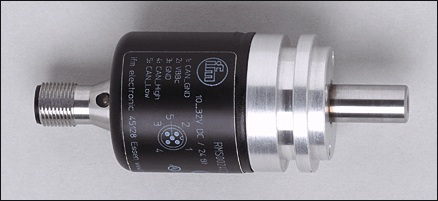
\includegraphics[width=1\columnwidth]{Encoder/foto}
 \caption{Encoder - RM9000 }
  
\end{figure}
\newpage

%\begin{figure}[h!]
 %\centering
 %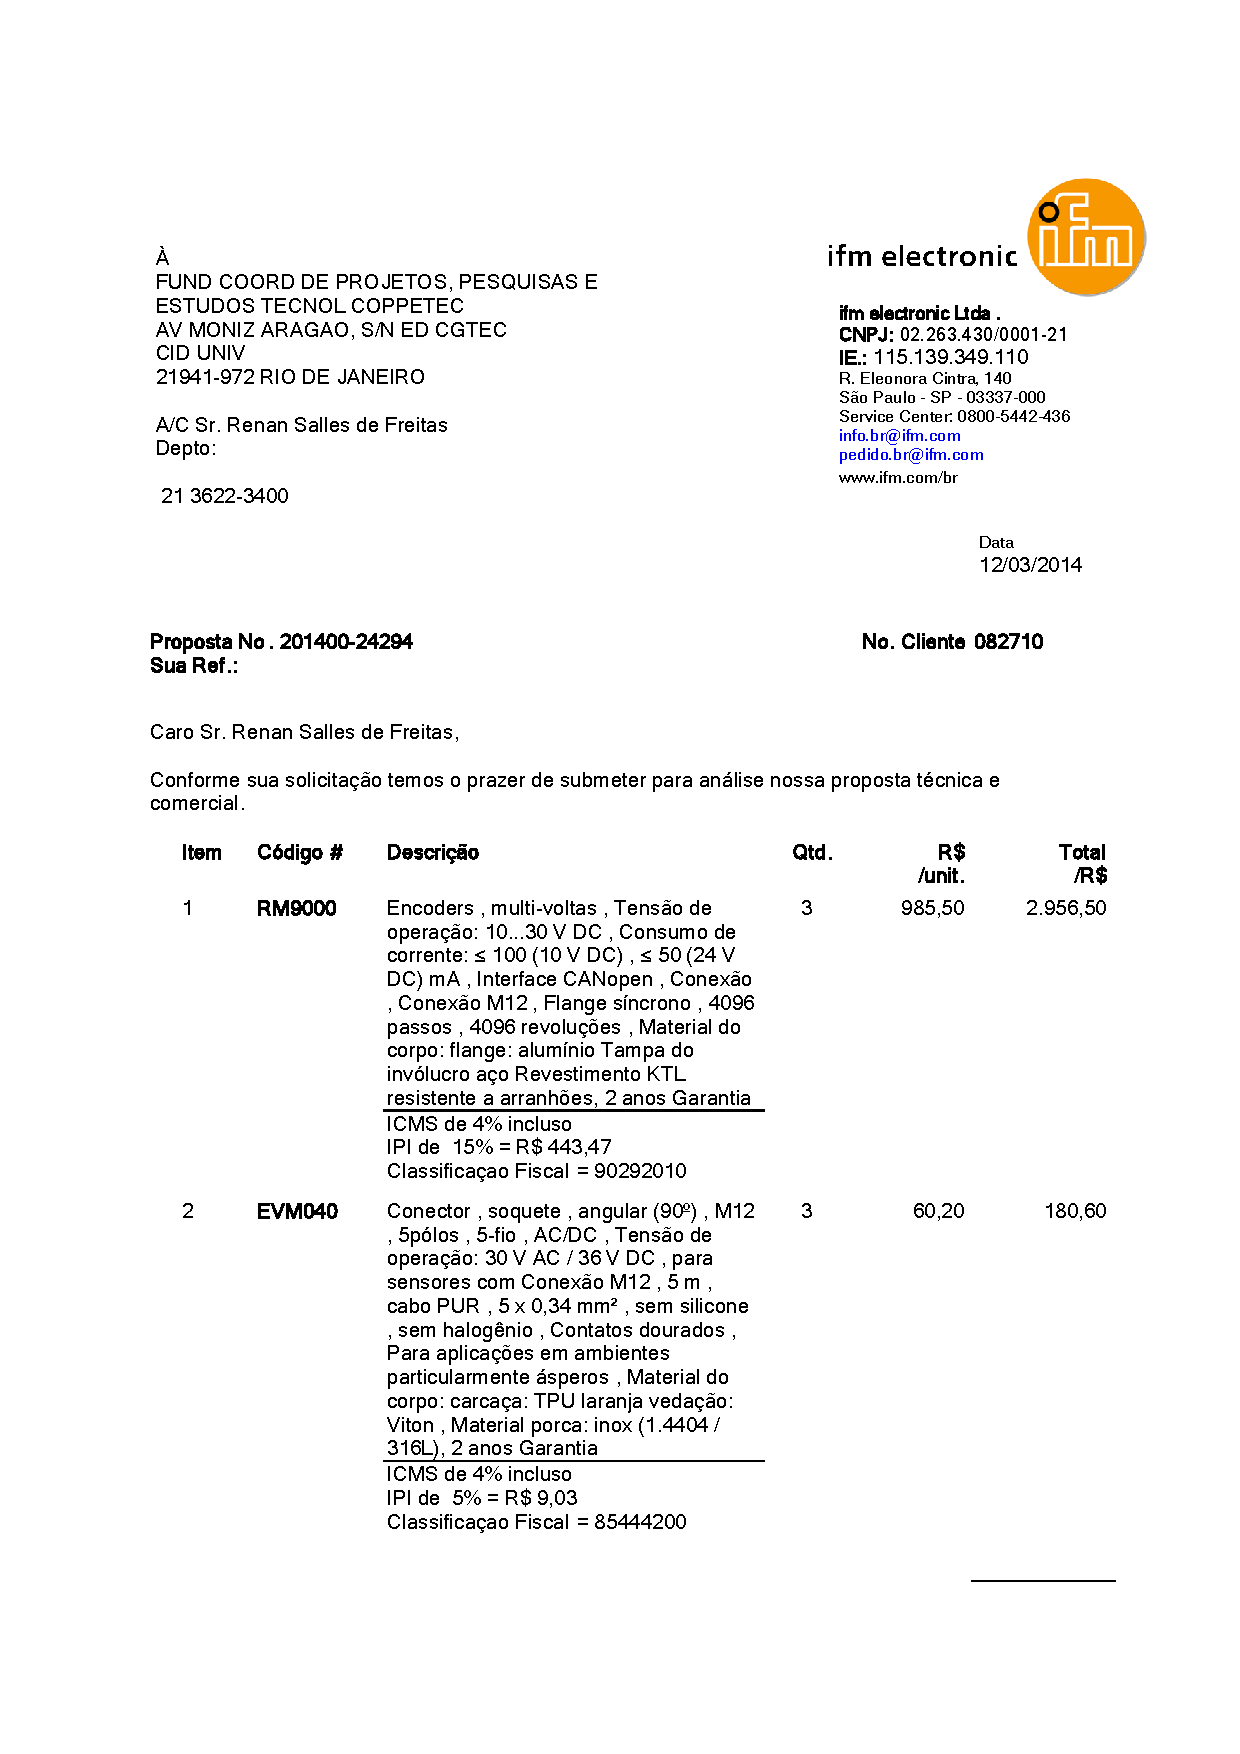
\includegraphics[width=1\columnwidth]{Encoder/price_quote_0.pdf}
 %\caption{Cotação RM9000 da IFM } 
%\end{figure}

\begin{figure}[h!]
 \centering
 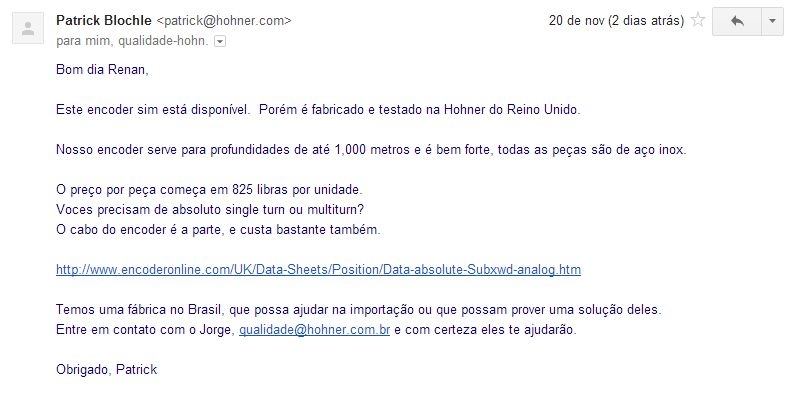
\includegraphics[width=1\columnwidth]{Encoder/price_quote_1}
 \caption{Cotação SUBXWD da Hohner}
\end{figure}

\begin{figure}[h!]
 \centering
 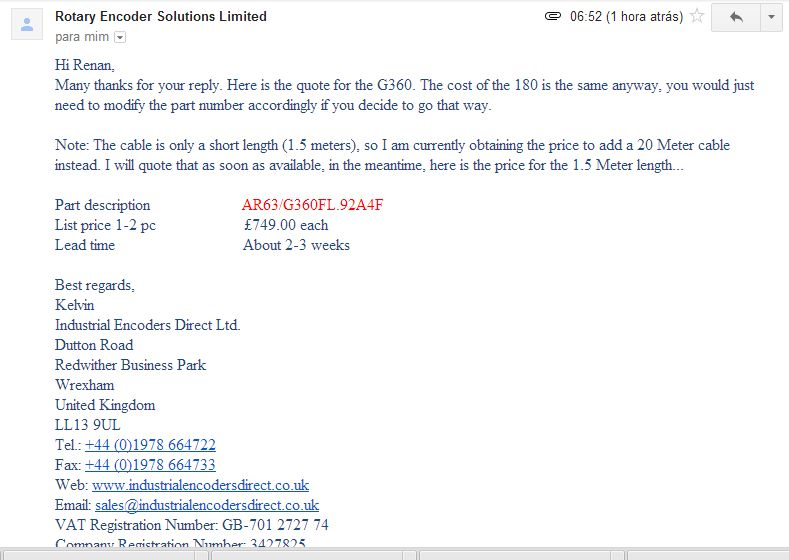
\includegraphics[width=1\columnwidth]{Encoder/price_quote_2}
 \caption{Cotação G360 da Rotay Encoder Solutions } 
\end{figure}